\section{The Environment of Distance Study}
\label{The Environment of Distance Study}
The Environment of Distance Study...

TODO pilt virtuaalaborite süsteemi kontekstist

\subsubsection{Random tags}
\begin{itemize}
	\item normal traffic generator
	\item malicious traffic generator
	\item availability monitor (for grading)
\end{itemize}

\subsubsection{Virtualization Layer}
Siin libvirdist
\subsubsection{Web Application Layer}
Siin Ruby on Rails raamistikust ja veebirakendusest

\subsection{Architecture of Distance Laboratory}
Siin räägin üldisest disainist ja allsüsteemidest
\
\begin{figure}[ht]
\centering
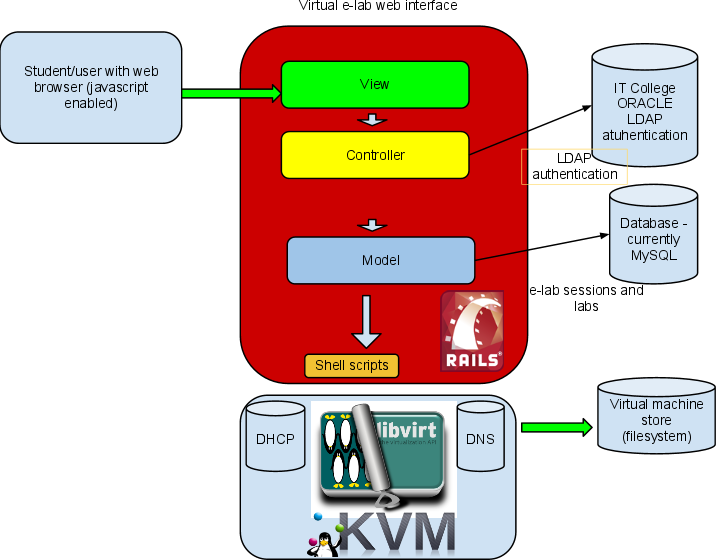
\includegraphics[width=0.8\textwidth]{architecture.png}
\caption{Architecture of Distance Laboratory}
\label{fig:Architecture of Distance Laboratory}
\end{figure}
\

\subsection{Security Aspects of Distance Laboratory}
